\documentclass[professionalfont, 12pt]{beamer} %, handout



%\usepackage{pxfonts}
%\usepackage{eulervm}

%\documentclass[sans,mathserif]{beamer}
%\usepackage{kerkis} % Kerkis roman and sans
%\usepackage{kmath}


%\documentclass[serif, professionalfont]{beamer} %
%\usepackage[T1]{fontenc} % Needed for Type1 Concrete
%\usepackage{concrete}


\usepackage{amsmath}
\usepackage{amsthm}
\usepackage{amsthm,amssymb,amsfonts,amsmath} 
% \usepackage{proof}
\usepackage[mathscr]{eucal}
\usepackage{amssymb,mathtools}
\usepackage{xcolor}
\usepackage{mathrsfs}
\usepackage{enumerate}
\usepackage{comment}

\usepackage{tikz}
\usetikzlibrary{shapes.geometric}
\usetikzlibrary{arrows}
\usetikzlibrary{shapes}
\usetikzlibrary{plotmarks}

 
 

\theoremstyle{plain}
\newtheorem{thm}{Theorem}
\newtheorem{remark}{Remark}
\newtheorem{cor}[thm]{Corollary}
 
\theoremstyle{definition}
\newtheorem{df}{Definition}
       
  
\usepackage{epsfig}
%\usepackage{amsmath}
%\usepackage{mathrsfs}
%\usepackage[all]{xy}  
%\usepackage{proof}    %%proof.style file
           

\newcommand{\tcb}[1]{\textcolor{blue}{#1}}
\newcommand{\tcr}[1]{\textcolor{red}{#1}}  
\newcommand{\tcc}[1]{\textcolor{cyan}{#1}}
\newcommand{\tcg}[1]{\textcolor{green}{#1}} 
\newcommand{\tcm}[1]{\textcolor{magenta}{#1}}      

\newcommand{\omt}{\mathop{\curlywedge}}
  
    
\newcommand{\Lra}{\: \Leftrightarrow \:}
\newcommand{\m}[1]{{\mathbf {#1} }}
%\newcommand{\m}[1]{{\mbox{\uppercase {\bf {#1}}}}}
%\newcommand{\N}[1]{{{ \m N_{#1}}}}
\newcommand{\Rl}{ {\mbox{$\mathcal{RL}  $}}}
\newcommand{\Rlc}{ {\mbox{$\mathcal{RL}^C  $}}}
\newcommand{\Ra}{{ \:\; \Rightarrow \:\; }}
%\newcommand{\Ra}{{\mbox{$ \: \Rightarrow \: $}}}
\newcommand{\Rar}{{ \: \Rightarrow \: }}
\newcommand{\La}{{\mbox{$ \: \Leftarrow \: $}}}
\newcommand{\ra}{\rightarrow}
\newcommand{\la}{\leftarrow}
\newcommand{\lra}{\leftrightarrow}
\newcommand{\fa}{\: \forall}
\newcommand{\lan}{(}
\newcommand{\ran}{)}
\newcommand{\rl}{{residuated lattice }}
\newcommand{\rls}{{residuated lattices }}
\newcommand{\T}{\top}
\newcommand{\jn}{\vee}
\newcommand{\mt}{\wedge}
\newcommand{\ror}{\: $ or $ \:}
\newcommand{\rand}{\: $ and $ \:}
\newcommand{\Tg}{\lan \T \ran}
\newcommand{\set}[2]{{\mbox{$ \{ #1 \: | \: #2 \}  $}}}
\newcommand{\ex}{\exists}
\newcommand{\eq}{\approx}
\newcommand{\eqv}{\cong}
\newcommand{\sbs}{\subseteq}
\newcommand{\sps}{\supseteq}
\newcommand{\vr}{{\mbox{$\mathcal{V}$}}}
\newcommand{\Vr}{{\mbox{$ \mathcal{V} \: $ }}}
\newcommand{\vrg}[1]{{\mbox{ $ \mathcal{V}  (\m #1) $}}}
\newcommand{\vs}{\emptyset}
\newcommand{\cov}{\prec}
\newcommand{\rd}{{/}}
\newcommand{\ld}{{\setminus}}
%\newcommand{\qed}{\hfill$\bullet$}
\newcommand{\ol}{\overline}
%\newcommand{\ua}{\hspace{.04in} \uparrow \hspace{-.04in}}
\newcommand{\ua}{\mathop{\uparrow}}
\newcommand{\da}{\hspace{.01in} \downarrow \hspace{-.01in}}
\newcommand{\dm}{\stackrel{\cdot}{-}}
\newcommand{\md}{\stackrel{-}{\cdot}}
\newcommand{\bra}{{\bf \ra}}
\newcommand{\blra}{{\bf \lra}}
\newcommand{\ban}{{\bf \&}}
\newcommand{\bor}{{\bf \nabla}}
\newcommand{\bmt}{{\bf \mt}}
\newcommand{\bjn}{{\bf \jn}}
\newcommand{\bneg}{{\bf \neg}}
\newcommand{\bbot}{{\bf \bot}}
\newcommand{\btop}{{\bf \top}}
\newcommand{\entails}{\vdash}
\newcommand{\TM}{{\mbox{{Turing Machine }}}}
\newcommand{\TMs}{{Turing Machines }}
\newcommand{\MM}{{Minskii Machine }}
\newcommand{\RA}{\Ra}
\newcommand{\rla}{{relation algebra }}
\newcommand{\rlas}{{relation algebras }}
\newcommand{\cv}{ ^{ \cup } }
\newcommand{\cg}{{\rm Cg}}                          %Petar
\newcommand{\var}[1]{{\uppercase \mathcal{{#1}}}}      %Petar
\newcommand{\Lg}{{\mbox{$\mathcal{LG} $}}}             %Partick
\newcommand{\Lgm}{{\mbox{$\mathcal{LG}^- $}}}          %Partick
\newcommand{\phibar}{{\mbox{$\ol \phi\ $}}}         %Partick
\newcommand{\vrm}{{\mbox{$\mathcal{V}^- $}}}           %Partick
\newcommand{\Ya}{\Rightarrow}
\newcommand{\bs}{\boldsymbol}
\newcommand{\cleq}{\preceq}
\newcommand{\hra}{\rightharpoonup}
\renewcommand{\ln}{\mathord{\sim}}
\newcommand{\rn}{\mathord{-}}
\newcommand{\lrh}{\mathop{\leftrightarrow}}
\providecommand{\semsb}{\ensuremath{\mathscr{M}}}
\providecommand{\sem}[1]{\ensuremath{\semsb (#1)}} 
\newcommand{\alhack}{\\[-\normalbaselineskip]\tag*{\qedhere}}
\providecommand{\psetsb}{\ensuremath{\mathscr{P}}}
\providecommand{\pset}[1]{\ensuremath{\psetsb (#1)}} 
\providecommand{\pfin}[1]{\ensuremath{\psetsb_{\text{fin}}(#1)}}

\newcommand{\co}{\mathsf} %fontshape for class operators
\newcommand{\cl}{\mathcal} %fontshape for general classes
\newcommand{\RL}{\va{RL}}
\DeclareMathOperator{\Mod}{Mod}
\newcommand{\bl}{\boldsymbol{\Lambda}}

% Macros for FL
\newcommand{\al}{\alpha}
\newcommand{\sig}{\Sigma}
\newcommand{\lam}{\Lambda}
\newcommand{\gam}{\Gamma}
\newcommand{\del}{\Delta}
\newcommand{\im}{\rightarrow}
\newcommand{\ya}{\rightarrow}
\newcommand{\naraba}{\rightarrow}
\newcommand{\To}{\vdash}
%\newcommand{\lan}{\left(} %not \la
%\newcommand{\ran}{\right)} %not \ra
%\newcommand{\Ya}{\Rightarrow}
\newcommand{\noi}{\noindent}
%\newcommand{\preast}{{\preceq}^{\ast}}
%\newcommand{\prestar}{{\preceq}^{\star}}
\newcommand{\epsi}{\varepsilon}
\newcommand{\e}{\varepsilon}

\newcommand{\p}{\vskip 12pt}
\newcommand{\q}{\vskip 6pt}


\newcommand{\btl}{\lhd}%{\triangleleft}{\blacktriangleleft}
\newcommand{\btr}{\rhd}%{\triangleright}{\blacktriangleright} 
\newcommand{\eb}[1]{\emph{\textcolor{blue}{#1}}}       
\newcommand{\cb}[1]{\textcolor{blue}{#1}} 
\newcommand{\cred}[1]{\textcolor{red}{#1}}        
\newcommand{\ldd}{\mathbin{\bbslash}}
\newcommand{\rdd}{\mathbin{\sslash}}  
\newcommand{\raa}{\mathbin{\leadsto}}    
\newcommand{\RarN}{{\sqsubseteq}}  %{{\mathrel{N}}} 
\newcommand{\RaN}{\mathnormal{\RarN}}

\newcommand{\va}{\mathsf} %fontshape for specific varieties  
\newcommand{\cnv}{u}

\renewcommand{\And}{\text{ \sf and }} %already exists in LaTeX
\newcommand{\Or}{\text{ \sf or }}
\newcommand{\AND}{\text{\sf{AND }}}
\newcommand{\bcdw}{\mbox{\boldmath{$\,\cdot\,$}}}


\renewcommand{\and}{\text{ \sf and }}
\newcommand{\orc}{\text{ \sf or }}
\newcommand{\orb}{\ \overline{\mbox{\sf or}}\ }
\newcommand{\Implies}{\Longrightarrow}
\providecommand{\undsc}{\underline{\phantom{x}}}

\newcommand{\gal}[1]{#1^+}

\newcommand{\force}{\vdash}
\def\hh{\ |\ }
\newcommand{\FL}{\mbox{$\mbox{\bf FL}$}}

\newcommand{\ls}{\setbox0\hbox{$-$}
\mathbin{\hbox{$-$\kern-\wd0\raise2\dp0\hbox{$\cdot$}\kern.3\wd0\lower2\dp0\hbox
{$\cdot$}}}}
\newcommand{\rs}{\setbox0\hbox{$-$}
\mathbin{\hbox{$-$\kern-\wd0\lower2\dp0\hbox{$\cdot$}\kern.3\wd0\raise2\dp0\hbox
{$\cdot$}}}}

\newcommand{\rdo}{\mathop{\mbox{$\bigcirc \! \! \! \! \! \rdd \, $}}}
\newcommand{\ldo}{\mathop{\mbox{$\bigcirc \! \! \! \! \! \ldd \, $}}}

%Lattices 
\providecommand{\MEET}{\ensuremath{\bigwedge}}
\providecommand{\Meet}{\ensuremath{\textstyle\bigwedge\limits}}
\providecommand{\Join}{\ensuremath{\bigvee}}
\providecommand{\meet}{\ensuremath{\wedge}}
\providecommand{\join}{\ensuremath{\vee}}

%Set Theory
\providecommand{\card}[1]{\ensuremath{\left\lvert#1\right\rvert}}
\providecommand{\intersect}{\ensuremath{\cap}}
\providecommand{\Intersect}{\ensuremath{\bigcap}}
\providecommand{\union}{\ensuremath{\cup}}
\providecommand{\UNION}{\ensuremath{\bigcup}}
\providecommand{\Union}{\ensuremath{\textstyle\bigcup\limits}}
%Logic
\providecommand{\iff}{\ensuremath{\Leftrightarrow}}
\providecommand{\implies}{\ensuremath{\Rightarrow}}

%Algebra
\providecommand{\normal}{\ensuremath{\unlhd}}
\providecommand{\embed}{\ensuremath{\hookrightarrow}}%inclusion map
\providecommand{\gen}[1]{\ensuremath{\left<#1\right>}}%Group generated by #1
\providecommand{\idx}[2]{\ensuremath{\left[#1:#2\right]}}%index of #2 in #1
\providecommand{\order}[1]{\ensuremath{\left\lvert#1\right\rvert}}

%Commonly used Sets
\providecommand{\C}{\ensuremath{\mathbb{C}}}%complex
\providecommand{\N}{\ensuremath{\mathbb{N}}}%natural
\providecommand{\Q}{\ensuremath{\mathbb{Q}}}%rationals
\providecommand{\R}{\ensuremath{\mathbb{R}}}%reals
\providecommand{\Z}{\ensuremath{\mathbb{Z}}}%integers
\providecommand{\Zpos}{\ensuremath{\mathbb{Z}^{+}}}%positive integers

%functions
\providecommand{\restrictedto}{\ensuremath{\downharpoonright}}

%Analysis and lineal algebra
\providecommand{\norm}[1]{\ensuremath{\left\lVert#1\right\rVert}}
\providecommand{\vect}{\ensuremath{\vec}}

%Miscellaneous
\providecommand{\abs}[1]{\ensuremath{\left\lvert#1\right\rvert}}
\providecommand{\define}{\ensuremath{\stackrel{\text{\tiny def}}{=}}}

%number theory
\providecommand{\floor}[1]{\ensuremath{\left\lfloor#1\right\rfloor}}
\providecommand{\ceil}[1]{\ensuremath{\left\lceil#1\right\rceil}}

%Miscellaneous shortcuts
\providecommand{\lcm}{\ensuremath{\text{lcm}}}%least common multiple
\providecommand{\st}{\ensuremath{\backepsilon}}

%Presentation dependant
\newcommand{\ccdot}{\bullet}

\newcommand\g[1]{g_{\bf{#1}}}
\newcommand\f[1]{f_{\bf{#1}}}
\newcommand{\gb}{\g{B}}
\newcommand{\gc}{\g{C}}
\newcommand{\fb}{\f{B}}
\newcommand{\fc}{\f{C}}


\usefonttheme[onlymath]{serif}
\usetheme{CambridgeUS} % My favorite!
%with an extra region at the top.
\useoutertheme[subsection=false]{miniframes}%smoothbars}
\definecolor{CrimsonRed}{rgb}{.5882,0,.1804} 
\definecolor{Gold}{rgb}{.6588,.6,.4313}
\definecolor{gold}{HTML}{997316}
\definecolor{Tan}{HTML}{BFB254}%{997316}
%\usecolortheme[named=Tan]{structure} %
%\setbeamercovered{invisible}
%\useoutertheme[right, width=1.8cm]{sidebar}
%\useinnertheme{circles}

\setbeamercolor{palette primary}{fg=CrimsonRed, bg=gold!45!white}
\setbeamercolor{palette sidebar primary}{fg=CrimsonRed} %, bg=gold!20!white}
\setbeamercolor{palette sidebar secondary}{fg=CrimsonRed!90!white}%, bg=gold!18!white}
\setbeamercolor{palette secondary}{fg=CrimsonRed, bg=Gold!30!white}
\setbeamercolor{palette tertiary}{fg=white!80!gold, bg=CrimsonRed}
\setbeamercolor{frametitle}{fg=CrimsonRed, bg=gold!05!white}
\setbeamercolor{title}{fg=gold!40!white, bg=CrimsonRed}
\setbeamercolor{item projected}{bg=Gold!70!white}
 \setbeamercolor{itemize item}{bg=Gold!20!white}
\setbeamertemplate{enumerate items}[default]
\setbeamercolor{block title}{fg=CrimsonRed,bg=gold!35!white}
\setbeamercolor{block body}{fg=black,bg=gold!7!white}
\setbeamercolor{local structure}{fg=Tan!50!white!70!black, }
\setbeamercolor{block title example}{bg=gold!30!white, fg=CrimsonRed}
\setbeamercolor{block body example}{bg=gold!07!white}
%\usecolortheme{sidebartab}

% To remove the navigation symbols from 
% the bottom of slides%
\setbeamertemplate{navigation symbols}{} 
%
\usepackage{graphicx}
%\usepackage{bm}         % For typesetting bold math (not \mathbold)%
%\titlegraphic{\includegraphics[height=1cm]{DU}}
%

\setbeamertemplate{caption}[numbered]
\DeclareMathOperator*{\bigor}{OR}
\newcommand{\bb}[1]{\mathbb {#1}}
\usepackage{setspace}

\title[Unilinear residuated lattices]{Unilinear residuated lattices}
\author[Xiao Zhuang]{Xiao Zhuang\\
  \small{joint work with Nick Galatos} }
\institute[University of Denver]
{University of Denver}
\date{BLAST 2023}
% \today will show current date. 
% Alternatively, you can specify a date.
% \titlegraphic{\includegraphics[]{}}
%BEAMER HACKS


%Backgroundcolor
%\setbeamercolor{background canvas}{bg=gold!09!white}



\begin{document}


%\begin{frame}[plain]
%\hspace*{1cm}\parbox[t]{\textwidth}{	
%\titlepage
%}
%\end{frame}


\begin{frame}[plain]{}
%\advance\textwidth1.7cm
\hsize\textwidth
\columnwidth\textwidth
\maketitle

\end{frame}

\section{Introduction}

\begin{frame}{Residuated lattices}
    A residuated lattice is an algebra $(R, \wedge, \vee, \cdot, \backslash, /, 1)$ where
    \begin{itemize}
        \item $(R, \wedge, \vee)$ is a lattice;

        \item $(R, \cdot, 1)$ is a monoid;

        \item For all $x, y, z \in R$,
        \begin{equation}\tag{residuation}\label{res.}
            x \cdot y \leq z \text{ iff } y \leq x \backslash z \text{ iff } x \leq z/x
        \end{equation}
    \end{itemize}

\pause

\begin{center}
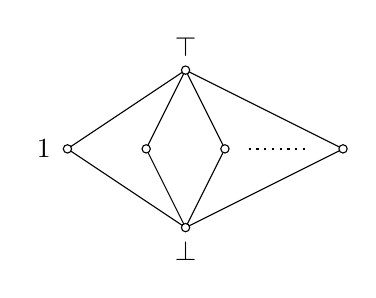
\begin{tikzpicture}
\draw (1.5, 1) -- (0, 0) -- (1.5, -1);
\draw (1.5, 1) -- (1, 0) -- (1.5, -1);
\draw (1.5, 1) -- (2, 0) -- (1.5, -1);
\draw (1.5, 1) -- (3.5, 0) -- (1.5, -1);
\draw[thick, dotted] (2.3, 0) -- (3.05, 0);

\filldraw [color = black, fill = white] (1.5, 1) circle (1.5pt)
(1.5, 1.3) node {$\top$};
\filldraw [color = black, fill = white] (1.5, -1) circle (1.5pt)
(1.5, -1.3) node {$\bot$};
\filldraw [color = black, fill = white] (0, 0) circle (1.5pt)
(-0.3, 0) node {$1$};
\filldraw [color = black, fill = white] (1, 0) circle (1.5pt);
\filldraw [color = black, fill = white] (2, 0) circle (1.5pt);
\filldraw [color = black, fill = white] (3.5, 0) circle (1.5pt);
\end{tikzpicture}
\end{center}

\end{frame}

\section{Residuated lattices on \texorpdfstring{$M_X$}{MX}}

\begin{frame}{Residuated lattices on $M_X$}
Given a set $X$, we denote by $\mathbf{M}_X$ the lattice over the set $X\cup \{\bot, \top\}$, where $\top$ is the top element, $\bot$ is the bottom element, and $x\vee y=\top$ and $x \wedge y=\bot$, for distinct $x,y \in X$.

\begin{figure}[h]
\centering
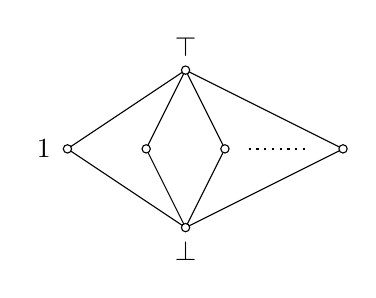
\begin{tikzpicture}
\draw (1.5, 1) -- (0, 0) -- (1.5, -1);
\draw (1.5, 1) -- (1, 0) -- (1.5, -1);
\draw (1.5, 1) -- (2, 0) -- (1.5, -1);
\draw (1.5, 1) -- (3.5, 0) -- (1.5, -1);
\draw[thick, dotted] (2.3, 0) -- (3.05, 0);

\filldraw [color = black, fill = white] (1.5, 1) circle (1.5pt)
(1.5, 1.3) node {$\top$};
\filldraw [color = black, fill = white] (1.5, -1) circle (1.5pt)
(1.5, -1.3) node {$\bot$};
\filldraw [color = black, fill = white] (0, 0) circle (1.5pt)
(-0.3, 0) node {$1$};
\filldraw [color = black, fill = white] (1, 0) circle (1.5pt);
\filldraw [color = black, fill = white] (2, 0) circle (1.5pt);
\filldraw [color = black, fill = white] (3.5, 0) circle (1.5pt);
\end{tikzpicture}
\caption{A residuated lattice over $M_X$}
\end{figure}
\end{frame}

\begin{frame}
    \begin{block}{A well-known result}
        The characterization of all residuated lattices based on $\mathbf{M}_X$ where $X$ is non-empty and closed under multiplication and $\bot$ is absorbing in $M_X$ and $\top$ is absorbing in $X \cup \{\top\}$ is known: $X$ is a cancellative monoid.
    \end{block}
    \pause
    
    A monoid $\mathbf{S}$ with a zero (absorbing element) $0$ is called \emph{$0$-cancellative} if for all $x, y, z \in S$,
    \begin{align*}
        xy = xz \neq 0 & \Rightarrow y = z\\
        yx = zx \neq 0 & \Rightarrow y = z.
    \end{align*}
    
\end{frame}

\begin{frame}{Properties}

In a residuated lattice $\bf{R}$ on $\mathbf{M}_X$, we define $U_R = \{x \in R \setminus \{\bot, \top\}: x \top = \top\}$ and $Z_R = \{x \in R \setminus \{\bot, \top\}: x \top = x\}$.
\pause

\begin{itemize}
    \item $\top$ is central in $\mathbf{R}$ and $R = U_R \sqcup Z_R \sqcup \{\bot, \top\}$.
    
    \item $U_{\top} = U_R \cup \{\top\}$ is a $\top$-cancellative submonoid of $\mathbf{R}$.
    
    \item $Z_{\bot} = Z_R \cup \{\bot\}$ is a subsemigroup of $\mathbf{R}$ with zero $\bot$, $|Z_{\bot}| \leq 3$ and $xy = \bot$ for all distinct $x, y \in Z_{\bot}$.\\    
    Also, either $Z_{\bot}$ is idempotent, or $Z_{\bot} = \{b, \bot\}$ with $b^2=\bot$.
    
    \item $ab = ba = b$ for all $a \in U_R$ and $b \in Z_R$.
\end{itemize}

\begin{figure}[h]
\centering
\scalebox{0.7}{
\begin{tabular}{c | c}
 & $\bot$\\
\hline
$\bot$ & $\bot$ 
\end{tabular}
,
\begin{tabular}{c | c c}
 & $\bot$ & $b$\\
\hline
$\bot$ & $\bot$ & $\bot$\\
$b$ & $\bot$ & $b$
\end{tabular}
,
\begin{tabular}{c | c c}
 & $\bot$ & $b$\\
\hline
$\bot$ & $\bot$ & $\bot$\\
$b$ & $\bot$ & $\bot$
\end{tabular}
,
\begin{tabular}{c | c c c}
 & $\bot$ & $b_1$ & $b_2$\\
\hline
$\bot$ & $\bot$ & $\bot$ & $\bot$\\
$b_1$ & $\bot$ & $b_1$ & $\bot$\\
$b_2$ & $\bot$ & $\bot$ & $b_2$ 	
\end{tabular}
}
\caption{Four multiplication tables of $Z_R$}
\label{f:4tables}
\end{figure}

\end{frame}

\begin{frame}{Construction and Characterization}

Let $\mathbf{A}$ be $\top$-cancellative monoid with zero $\top$ and $\mathbf{B}$ be a semigroup with zero $\bot$, whose multiplication table is one of those in Figure~\ref{f:4tables}.\pause
We define the lattice structure $\mathbf{M}_X$ on the set $R = A \cup B$, where $X = R \setminus \{\bot, \top\}$, $\bot$ is the bottom and $\top$ is the top. \pause
Also, we define a multiplication on $R$ that extends the multiplications on $\mathbf{A}$ and $\mathbf{B}$ by: $xy = yx = y$, for all $x \in A$ and $y \in B$.
We denote by $\mathbf{R}_{\mathbf{A}, \mathbf{B}}$ the resulting algebra.
\end{frame}

\begin{frame}
\begin{block}{Theorem}
    $\mathbf{R}_{\mathbf{A}, \mathbf{B}}$ is the reduct of a residuated lattice based on $\mathbf{M}_X$, where $X = A \cup B \setminus \{\bot, \top\}$.
\end{block}
\pause

\begin{block}{Corollary}
    The residuated lattices based on $\mathbf{M}_X$ are precisely the ones of the form $\mathbf{R}_{\mathbf{A}, \mathbf{B}}$, where $\mathbf{A}$ is a $\top$-cancellative monoid with zero $\top$ and $\mathbf{B}$ is a semigroup with zero $\bot$, whose multiplication table is one of those in Figure~\ref{f:4tables}; and integral ones: $2$-element Boolean algebra, $3$-element Heyting algebra, $3$-element MV-algebra and $4$-element Boolean algebra.
\end{block}
\end{frame}

\section{Axiomatization}

\begin{frame}{Axiom (URL)}
    A residuated lattice is called \emph{unilinear} if it satisfies 
    \begin{equation}\tag{URL}\label{axiom_URL}
        \begin{split}
            \forall u_1, u_2, z, w \, \, (u_1 \leq u_2 & \text{ or } u_2 \leq u_1\\
            & \text{ or } (u_1 \wedge u_2 \leq w \text{ and } z \leq u_1 \vee u_2)).
        \end{split}        
    \end{equation}

    %Need to talk about the difference between linear and non-linear cases and the impact of this axiom about linear ones

    \pause
    
    \begin{center}
    \scalebox{0.5}{
    \begin{tikzpicture}
        \draw (3, 4) -- (0, 3);
        \draw[dotted] (0, 3) -- (0, -3);
        \draw (0, -3) -- (3, -4);
        \draw (3, 4) -- (1.5, 3);
        \draw[dotted] (1.5, 3) -- (1.5, -3);
        \draw (1.5, -3) -- (3, -4);
        \draw[dotted] (2, 0) -- (5.5, 0);
        \draw (3, 4) -- (6, 3);
        \draw[dotted] (6, 3) -- (6, -3);
        \draw (6, -3) -- (3, -4);

        \filldraw [color = black, fill = white] (3, 4) circle (2.5pt)
            (3, 4.4) node {$\top$};
        \filldraw [color = black, fill = white] (3, -4) circle (2.5pt)
            (3, -4.4) node [black] {$\bot$};
        \filldraw [color = black, fill = white] (0, 2) circle (2.5pt)
            (-0.3, 2.3) node [black] {};
        \filldraw [color = black, fill = white] (0, 1) circle (2.5pt)
            (-0.3, 1.3) node [black] {};
        \filldraw [color = black, fill = white] (0, 0) circle (2.5pt)
            (-0.3, 0.3) node [black] {};
        \filldraw [color = black, fill = white] (0, -1) circle (2.5pt)
            (-0.4, -0.7) node [black] {};
        \filldraw [color = black, fill = white] (0, -2) circle (2.5pt)
            (-0.4, -1.7) node [black] {};

        \filldraw [color = black, fill = white] (1.5, 2) circle (2.5pt);
        \filldraw [color = black, fill = white] (1.5, 1) circle (2.5pt);
        \filldraw [color = black, fill = white] (1.5, 0) circle (2.5pt)
            (1.2, 0.3) node {};
        \filldraw [color = black, fill = white] (1.5, -1) circle (2.5pt);
        \filldraw [color = black, fill = white] (1.5, -2) circle (2.5pt);

        \filldraw [color = black, fill = white] (6, 2) circle (2.5pt);
        \filldraw [color = black, fill = white] (6, 1) circle (2.5pt);
        \filldraw [color = black, fill = white] (6, 0) circle (2.5pt)
            (6.3, 0.3) node [black] {};
        \filldraw [color = black, fill = white] (6, -1) circle (2.5pt);
        \filldraw [color = black, fill = white] (6, -2) circle (2.5pt);
    \end{tikzpicture}
    }
    \end{center}

\end{frame}

\begin{frame}{Axiom ($h_n$)}

    A (bounded) residuated lattice has height at most $n$ iff it satisfies
    \begin{equation}\tag{$h_n$}\label{axiom_of_finite_height}
            \forall x_1, \dots, x_{n+1} \, (\bigor \limits_{1 \leq m \leq n}
            x_1 \vee \dots \vee x_{m} = x_1 \vee \dots \vee x_{m+1}).
    \end{equation}

    In particular, $(h_3)$ is the universal closure of 
    $$x_1 = x_1 \vee x_2 \text{ or } x_1 \vee x_2 = x_1 \vee x_2 \vee x_3 \text{ or } x_1 \vee x_2 \vee x_3 = x_1 \vee x_2 \vee x_3 \vee x_4.$$

    \pause

    \begin{block}{Corollary}
        The residuated lattices on $\mathbf{M}_X$ are precisely the ones in the class $\mathsf{URL}_3$.
    \end{block}
\end{frame}

\section{Equational basis}

\begin{frame}{Equations for (URL)}
Given the positive universal sentence
\begin{align*}
    \forall u_1, u_2, z, w \, \, (u_1 \leq u_2 & \text{ or } u_2 \leq u_1\\
            & \text{ or } (u_1 \wedge u_2 \leq w \text{ and } z \leq u_1 \vee u_2)),
\end{align*}
we have

\begin{block}{[Gal04]}
    The variety $\mathsf{SRL}$ of semiunilinear residuated lattices is axiomatized by the infinitely many equations 
    \begin{align*}
        1 & = \gamma_1(x \backslash y) \vee \gamma_2(y \backslash x) \vee \gamma_3 ((x \wedge y) \backslash z)\\
        1 & = \gamma_4(x \backslash y) \vee \gamma_5(y \backslash x) \vee \gamma_6 (w \backslash (x \vee y)),
    \end{align*}
    where $ \gamma_1, \gamma_2, \gamma_3, \gamma_4, \gamma_5, \gamma_6 \in \Gamma(X)$ and $X$ is the set of variables.
\end{block}
\end{frame}

\begin{frame}{Equations for $(h_3)$}
Similarly, given the sentence
\begin{align*}
    \forall x_1, x_2, x_3, x_4 \, (x_1 = x_1 \vee x_2 & \text{ or } x_1 \vee x_2 = x_1 \vee x_2 \vee x_3\\
    & \text{ or } x_1 \vee x_2 \vee x_3 = x_1 \vee x_2 \vee x_3 \vee x_4)
\end{align*}
we get
\begin{block}{}
    The variety $\mathsf{M}$ generated by the class $\mathsf{URL}_3$, of residuated lattices on an $\mathbf{M}_X$, is axiomatized by the semiunilinear equations together with the equations 
    \begin{align*}
        1 = \gamma_1((x_1 \vee x_2)\backslash x_1) \vee & \gamma_2((x_1 \vee x_2 \vee x_3)\backslash (x_1 \vee x_2))\\
        \vee & \gamma_3((x_1 \vee x_2 \vee x_3 \vee x_4) \backslash (x_1 \vee x_2 \vee x_3)),
    \end{align*}
    where $\gamma_1, \gamma_2, \gamma_3 \in \Gamma(X)$ and $X$ is the set of variables.
\end{block}

\end{frame}

\begin{frame}{Finitely subdirectly irreducible algebras}
    \begin{block}{Theorem [Gal04]}
        Let $\varphi$ be an open positive universal formula in the language of residuated lattices and $\m L$ a residuated lattice.
        If $\m L$ is finitely subdirectly irreducible, then $\m L$ satisfies $(\forall \overline{x})(\varphi(\overline{x}))$ iff $\m L$ satisfies the equation $\forall \overline{x}, \overline{y} (\varepsilon(\overline{x}, \overline{y}))$, for all $\varepsilon(\overline{x}, \overline{y}) \in B_Y(\varphi'(\overline{x}))$ and $\overline{y} \in Y^l$, for some appropriate $l \in \bb{N}$.
    \end{block}
    \pause
    
    \begin{block}{Theorem}
        The finitely subdirectly irreducible (FSI) semiunilinear residuated lattices are precisely the unilinear residuated lattices: $\mathsf{SRL_{FSI}} = \mathsf{URL}$.
        More generally, if $\phi$ is a set of positive universal sentences, then all the FSIs in  $\mathsf{SRL} \cap \mathsf{V}_\phi$ are precisely the unilinear residuated lattices that satisfy $\phi$.
    \end{block}

\end{frame}

\begin{frame}{}
    \begin{block}{Corollary}
        The subdirectly irreducibles in $\mathsf{M}$ are the same as the finitely subdirectly irreducible in $\mathsf{M}$ and they are precisely the non-trivial residuated lattices based on $\mathbf{M}_X$.
    \end{block}
\end{frame}

\section{Subvarieties of \texorpdfstring{$\mathsf{M}$}{M}}

\begin{frame}{Subvarieties of $\mathsf{M}$}
There are uncountably many subvarieties of $\mathsf{M}$. \pause
More precisely, the variety $\mathsf{CM_G}$ generated by all the residuated lattices of the form $\mathbf{M}_{\mathbf{G}}$, where $\mathbf{G}$ is an abelian group, has uncountably-many subvarieties.
Actually, we give a full description of the subvariety lattice of $\mathsf{CM}_{\mathbf{G}}$.

\begin{block}{Theorem}
    The subvariety lattice of $\mathsf{CM}_{\mathbf{G}}$ is isomorphic to $\mathcal{O}_{\mathbb{Z}}(\m P)$.
\end{block}
\end{frame}

\begin{frame}{Lattice $\m P$ and $\bb{Z}$-closed downsets}
    $\bb{N}^\omega:$ direct power of countably many copies of the chain $(\mathbb{N}, \leq)$.
    
    $I \subseteq \bb{N}^\omega:$ lattice of (not necessarily strictly) decreasing sequences that are eventually zero, such as $(4, 2, 1, 1, 0, 0, \dots)$, $(3, 2, 1, 1, 1, 0, 0, \dots)$ etc. (we use $(4, 2, 1, 1)$ and $(3, 2, 1, 1, 1)$ to denote them)
    
    $I^{\oplus \omega} \subseteq \m I^\omega:$ lattice of all sequences of elements of $I$ that are eventually the zero sequence, e.g., $(2, 1; 3, 1, 1; 0; 2, 1, 1; 0; \dots)$.
    
    $\m{P} := \m 2 \times \m I^{\oplus \omega}$, where $\m 2$ is the two element lattice on $\{0,1\}$.\pause
    
    For $a \in P$, we define $\text{exp}(a)$ to be the maximum number appearing in $a$; e.g., $\text{exp}(1; 2, 1; 3; 0; 2,; 0; \dots) = 3$ and $\text{exp}(0; 1; 4, 1; 0; \dots) = 4$.
    Also, for $a \in P$ we write $a = (a_0; a_1; a_2; \ldots)$, where $a_0 \in \{0, 1\}$ and $a_n \in I$, for $n > 0$; we define $\text{prime}(a) = \{n \in \bb{N}: a_n \neq \overline{0}\}$.
    For $T \subseteq P$, we define $\text{exp}(T) = \{\text{exp}(a): a \in T\}$ and $\text{prime}(T) = \bigcup \{\text{prime}(a): a \in T\}$.
\end{frame}

\begin{frame}{Lattice $\m P$ and $\bb{Z}$-closed downsets}
A downset $D$ of $\m{P}$ is said to be \emph{$\bb{Z}$-closed} if for all $a \in P$, 
\begin{center}
$\text{exp}(D \cap {\uparrow} a)$ or $\text{prime}(D \cap {\uparrow} a)$ is unbounded implies $a \jn (1; 0; 0; \ldots) \in D$.
\end{center}
 
For example, for $a = (0;1;0;0;0;...)$, this condition has the following consequences:
$(0;1;1;0;0;\ldots), (0;1;2;0;0;\ldots), (0;1;3;0;0;\ldots), \ldots \in D$
or
$(0;1,1;0;0;\ldots), (0;2,1;0;0;\ldots), (0;3,1;0;0;\ldots), \ldots \in D$
implies $(1;1;0;0;0;\ldots) \in D$, because $\text{exp}(D \cap {\uparrow} a)$ is unbounded.
\pause
Also,
$(0;1;1;0;0;\ldots), (0;1;0;1;0;\ldots), (0;1;0;0;1;\ldots), \ldots \in D$
implies $(1;1;0;0;0;\ldots) \in D$, because $\text{prime}(D \cap {\uparrow} a)$ is unbounded.\pause
However,
$(0;1;1;0;0;\ldots), (0;1;1,1;0;0;\ldots), (0;1;1,1,1;0;0;\ldots), \ldots \in D$
does not imply $(1;1;0;0;0;\ldots) \in D$.

We denote the lattice of all $\bb{Z}$-closed downsets of $\m{P}$ by $\mathcal{O}_{\bb{Z}}(\m{P})$.
\end{frame}

\begin{comment}
\begin{frame}{Sketch of the proof}
    \begin{block}{}
        The lattice of subvarieties of $\mathsf{CM}_{\mathbf{G}}$ is isomorphic to the lattice of  $\mathsf{HSP_U}$-classes of FSIs in $\mathsf{CM}_{\mathbf{G}}$, which are $\mathsf{HSP_U}$-classes of algebras of the form $\m{M}_{\m{G}}$, where $\m{G}$ is an abelian group.
    \end{block}
    \begin{block}{}
        The $\mathsf{HSP_U}$-classes of $\m {M_G}$'s are actually $\mathsf{ISP_U}$-classes.
        The lattice of $\mathsf{ISP_U}$-classes of $\m {M_G}$'s is isomorphic to the lattice of $\mathsf{ISP_U}$-classes of abelian groups.
    \end{block}
    \begin{block}{}
        $\mathsf{ISP_U}$-classes of abelian groups are fully determined by their intersection with the class of finitely generated abelian groups.
    \end{block}
\end{frame}

\begin{frame}
\frametitle{Sketch of the proof}
    \begin{block}{Fundamental theorem of finitely generated abelian groups}
        Every finitely generated abelian group is isomorphic to exactly one group of the form
        \[
            \mathbb{Z}^m \times (\mathbb{Z}_{p_1^{n_{p_1, 1}}} \times \cdots \times \mathbb{Z}_{p_1^{n_{p_1,m_1}}}) \times \cdots \times (\mathbb{Z}_{p_k^{n_{p_k, 1}}} \times \cdots \times \mathbb{Z}_{p_k^{n_{p_k,m_k}}})  
        \]
        for some $k, m, m_1, \dots, m_k,n_{p_i,j} \in \mathbb{N}$, where $n_{i,j} \geq n_{i,j+1}$ for all suitable $j,j$, and $p_1 < p_2< \dots < p_k < \ldots $ is the listing of all primes.
    \end{block}
    Denote by $\mathcal{FA}$ the set of all groups of this form.
    \begin{block}{}
        The lattice of $\mathsf{ISP_U}$-classes of abelian groups is the same as the lattice of the intersections of $\mathsf{ISP_U}$-classes of abelian groups and $\mathcal{FA}$, i.e., the lattice of $\mathcal{K}_{\mathcal{FA}}$.
    \end{block}
\end{frame}

\begin{frame}{Sketch of the proof}
    \begin{block}{}
        $\m G \times \mathbb{Z}^r \in \mathcal{K}$ iff $\m G \times \mathbb{Z}^s \in \mathcal{K}$ for $r, s \in \bb{Z}^+$, $\m G \in \mathcal{FA}_{\text{fin}}$ and $\mathcal{K}$ an $\mathsf{ISP_U}$-class of abelian groups.
    \end{block}
    \pause
    \begin{block}{}
        The lattice of $\mathcal{K}_{\mathcal{FA}}$ is isomorphic to the lattice of $\mathcal{K}_{\mathcal{FA}'}$, where $\mathcal{FA}' = \{\m G, \bb{Z} \times \m G: \m G \in \mathcal{FA}_{\text{fin}}\}$.
    \end{block}
    \pause
    \begin{block}{}
    $\mathcal{FA}'$ is isomorphic to $\m P = \m 2 \times \m I^{\oplus \omega}$.
    \end{block}
    \begin{block}{Theorem}
    The subvariety lattice of $\mathsf{CM}_{\mathbf{G}}$ is isomorphic to $\mathcal{O}_{\mathbb{Z}}(\m P)$.
\end{block}
\end{frame}
\end{comment}

\begin{frame}
\begin{block}{Corollary}
    The variety generated by $\{\m M_{\mathbb{Z}_p}: p \text{ is prime}\}$ has uncountably many subvarieties. 
    Therefore the subvariety lattices of $\mathsf{M_G}$ and of $\mathsf{M}$ have size continuum.
\end{block}
\pause

We denote by $\mathsf{CM_{GZ}}$ the variety generated by the algebras in $\mathsf{M}$ that satisfy the formula $x \overline{\top} = x \text{ or } x(x \ld 1) = 1$.

Let $\m F$ be the poset on $\{0,1,2,3\}$, where $0 < 1, 2, 3$ and $1, 2, 3$ are incomparable.
For a downset $D$ of $\m P \times \m F$ and $i \in F$, we set $D_i = \{a: (a, i) \in D\}$. 
A downset $D$ of $\m P \times \m F$ is called $\mathbb{Z}$-closed if $D_0$, $D_1$, $D_2$ and $D_3$ are $\mathbb{Z}$-closed downsets of $\m P$; we denote by $\mathcal{O}_{\mathbb{Z}}(\m P \times \m F)$ the lattice of all $\mathbb{Z}$-closed downsets of $\m P \times \m F$.

\begin{block}{Corollary}
The subvariety lattice of $\mathsf{CM_{GZ}}$ is isomorphic to $\mathcal{O}_{\mathbb{Z}}(\m P \times \m F)$.
\end{block}
    
\end{frame}

\section{Constructing compact URL}

\begin{frame}{Compact URL}
    Let $\m R$ be a unilinear residuated lattice.
    If $\m R$ satisfies the formula
    \[
        u \leq v \text{ or } v \leq u \text{ or } x = u \mt v \text{ or } x(u \jn v) = (u \jn v)x = u \jn v
    \]
    and
    \[
        u \leq v \text{ or } v \leq u \text{ or } x = u \jn v \text{ or } x(y \mt z) = xy \mt xz,
    \]
    then we call $\m R$ is compact.

    Note if $\m R$ is bounded, being compact is equivalent to
    \[
        x = \bot \text{ or } x \top = \top x = \top
    \]
    and
    \[
        x = \top \text{ or } x (y \mt z) = xy \mt xz.
    \]

    $\m M_{\m G}$ is a compact URL, but there exists $\m {M_X}$ being not compact.
\end{frame}

\begin{frame}{Finite cyclic monoid}
    Given a finite cyclic monoid $\mathbf{M}$ generated by $a \in M$, there is a smallest natural number $r$, called the \emph{index}, such that $a^r = a^{r+s}$ for some  positive integer $s$; the smallest such $s$ then is called the \emph{period}.
    So $M = \{1, a, \dots, a^r, \dots, a^{r+s-1}\}$ and $|M|=r+s$.\pause
    
    Note that every natural number $n > r$ can be written as $n=r+ms+k$ for unique $m \in \mathbb{N}$ and $0 \leq k <s$; we define $[n]_r^s:= r+k$ for $n \geq r+s$ and $[n]_r^s:= n$ for $0 \leq n < r+s$.
    (We will write $[n]$, when $r,s$ are clear from the context.)
    Then the multiplication on $\m M$ is given by $a^i \cdot a^j =a^{[i+j]_r^s}$.
    In particular, $\{a^r, \dots, a^{r+s-1}\}$ is a subsemigroup of $\m M$ and it is a  group in its own right with identity element $a^t$ such that $t \equiv 0 \, (\text{mod } s)$; so it is isomorphic to $\mathbb{Z}_s$.
\end{frame}

\begin{frame}{Compact URL: $\m R_{\m M}$}
    We extend the multiplication of $\m M$ to the set $R = M \cup \{\bot, \top\}$ by $\bot x = x \bot = \bot$ for all $x \in R$, and $\top x = x \top = \top$ for all $x \not = \bot$.
    Also we define an order on $R$ by $\bot \leq x \leq \top$ for all $x \in R$ and
    $a^i \leq a^j$ if and only if $j = i+ns$ for some $0 \leq n \leq \lfloor (r+s-1-i)/s \rfloor$, for all $0 \leq i, j \leq r+s-1$.
    It is easy to see that this yields a unilinear lattice order.
    We denote by $\m R_{\m M}$ the resulting lattice-ordered monoid.

    \begin{block}{}
        If $\m M$ is a finite cyclic monoid, then $\mathbf{R}_{\m M}$ is the reduct of a resiudated lattice.
    \end{block}
    \pause

    Actually, we can prove that given a finite cyclic monoid $M$, there are only two lattices over which $\m R_{\m M}$ is a reduct of a compact URL.
\end{frame}

\begin{frame}
\begin{figure}[ht]
\centering
\scalebox{0.7}{
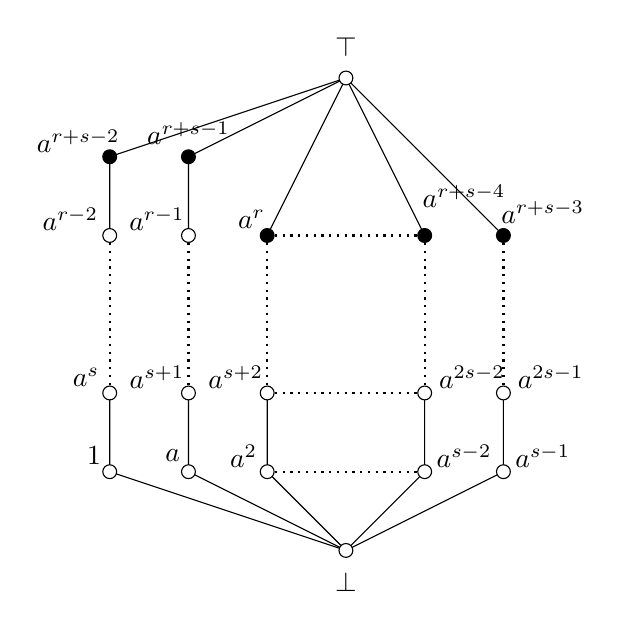
\begin{tikzpicture}
\draw (3, 3) -- (0, 2) -- (0, 1);
\draw [thick, dotted] (0, 1) -- (0, -1);
\draw (0, -1) -- (0, -2) -- (3, -3);
\draw (3, 3) -- (1, 2) -- (1, 1);
\draw [thick, dotted] (1, 1) -- (1, -1);
\draw (1, -1) -- (1, -2) -- (3, -3);
\draw (3, 3) -- (2, 1);
\draw [thick, dotted] (2, 1) -- (2, -1);
\draw (2, -1) -- (2, -2) -- (3, -3);
\draw [thick, dotted] (2, 1) -- (4, 1);
\draw [thick, dotted] (2, -1) -- (4, -1);
\draw [thick, dotted] (2, -2) -- (4, -2);
\draw (3, 3) -- (4, 1);
\draw [thick, dotted] (4, 1) -- (4, -1);
\draw (4, -1) -- (4, -2) -- (3, -3);
\draw (3, 3) -- (5, 1);
\draw [thick, dotted] (5, 1) -- (5, -1);
\draw (5, -1) -- (5, -2) -- (3, -3);

\filldraw [color = black, fill = white] (3, 3) circle (2.5pt)
    (3, 3.4) node {$\top$};
\filldraw [color = black, fill = white] (3, -3) circle (2.5pt)
    (3, -3.4) node {$\bot$};
\filldraw [color = black, fill = black] (0, 2) circle (2.5pt)
    (-0.4, 2.2) node {$a^{r+s-2}$};
\filldraw [color = black, fill = white] (0, 1) circle (2.5pt)
    (-0.5, 1.2) node {$a^{r-2}$};
\filldraw [color = black, fill = white] (0, -1) circle (2.5pt)
    (-0.3, -0.8) node {$a^s$};
\filldraw [color = black, fill = white] (0, -2) circle (2.5pt)
    (-0.2, -1.8) node {$1$};
    
\filldraw [color = black, fill = black] (1, 2) circle (2.5pt)
    (1, 2.3) node {$a^{r+s-1}$};
\filldraw [color = black, fill = white] (1, 1) circle (2.5pt)
    (0.6, 1.2) node {$a^{r-1}$};
\filldraw [color = black, fill = white] (1, -1) circle (2.5pt)
    (0.6, -0.8) node {$a^{s+1}$};
\filldraw [color = black, fill = white] (1, -2) circle (2.5pt)
    (0.8, -1.8) node {$a$};
    
\filldraw [color = black, fill = black] (2, 1) circle (2.5pt)
    (1.8, 1.2) node {$a^r$};
\filldraw [color = black, fill = white] (2, -1) circle (2.5pt)
    (1.6, -0.8) node {$a^{s+2}$};
\filldraw [color = black, fill = white] (2, -2) circle (2.5pt)
    (1.7, -1.8) node {$a^2$};
    
\filldraw [color = black, fill = black] (4, 1) circle (2.5pt)
    (4.5, 1.5) node {$a^{r+s-4}$};
\filldraw [color = black, fill = white] (4, -1) circle (2.5pt)
    (4.6, -0.8) node {$a^{2s-2}$};
\filldraw [color = black, fill = white] (4, -2) circle (2.5pt)
    (4.5, -1.8) node {$a^{s-2}$};
    
\filldraw [color = black, fill = black] (5, 1) circle (2.5pt)
    (5.5, 1.3) node {$a^{r+s-3}$};
\filldraw [color = black, fill = white] (5, -1) circle (2.5pt)
    (5.6, -0.8) node {$a^{2s-1}$};
\filldraw [color = black, fill = white] (5, -2) circle (2.5pt)
    (5.5, -1.8) node {$a^{s-1}$};
\end{tikzpicture}
\qquad
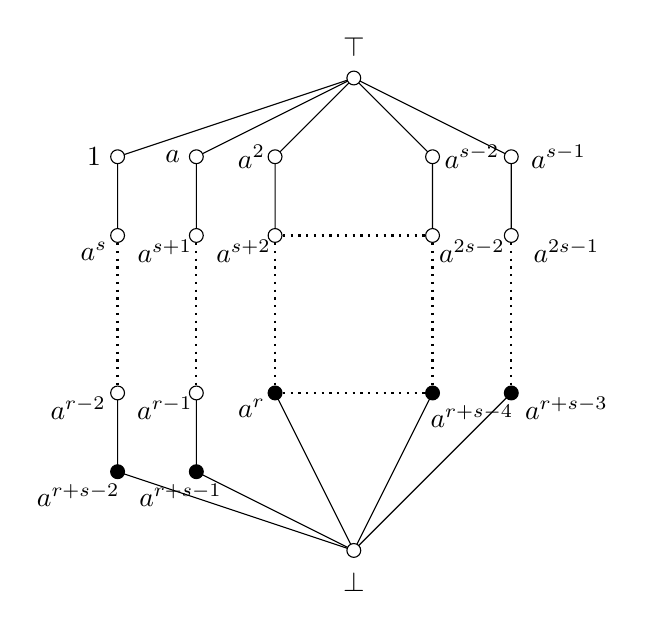
\begin{tikzpicture}
\draw (3, 3) -- (0, 2) -- (0, 1);
\draw [thick, dotted] (0, 1) -- (0, -1);
\draw (0, -1) -- (0, -2) -- (3, -3);
\draw (3, 3) -- (1, 2) -- (1, 1);
\draw [thick, dotted] (1, 1) -- (1, -1);
\draw (1, -1) -- (1, -2) -- (3, -3);
\draw (3, 3) -- (2, 2) -- (2, 1);
\draw [thick, dotted] (2, 1) -- (2, -1);
\draw (2, -1) -- (3, -3);
\draw [thick, dotted] (2, 1) -- (4, 1);
\draw [thick, dotted] (2, -1) -- (4, -1);
\draw (3, 3) -- (4, 2) -- (4, 1);
\draw [thick, dotted] (4, 1) -- (4, -1);
\draw (4, -1) -- (3, -3);
\draw (3, 3) -- (5, 2) -- (5, 1);
\draw [thick, dotted] (5, 1) -- (5, -1);
\draw (5, -1) -- (3, -3);

\filldraw [color = black, fill = white] (3, 3) circle (2.5pt)
    (3, 3.4) node {$\top$};
\filldraw [color = black, fill = white] (3, -3) circle (2.5pt)
    (3, -3.4) node {$\bot$};
\filldraw [color = black, fill = white] (0, 2) circle (2.5pt)
    (-0.3, 2) node {$1$};
\filldraw [color = black, fill = white] (0, 1) circle (2.5pt)
    (-0.3, 0.8) node {$a^s$};
\filldraw [color = black, fill = white] (0, -1) circle (2.5pt)
    (-0.5, -1.2) node {$a^{r-2}$};
\filldraw [color = black, fill = black] (0, -2) circle (2.5pt)
    (-0.5, -2.3) node {$a^{r+s-2}$};
    
\filldraw [color = black, fill = white] (1, 2) circle (2.5pt)
    (0.7, 2) node {$a$};
\filldraw [color = black, fill = white] (1, 1) circle (2.5pt)
    (0.6, 0.8) node {$a^{s+1}$};
\filldraw [color = black, fill = white] (1, -1) circle (2.5pt)
    (0.6, -1.2) node {$a^{r-1}$};
\filldraw [color = black, fill = black] (1, -2) circle (2.5pt)
    (0.8, -2.3) node {$a^{r+s-1}$};
    
\filldraw [color = black, fill = white] (2, 2) circle (2.5pt)
    (1.7, 2) node {$a^2$};
\filldraw [color = black, fill = white] (2, 1) circle (2.5pt)
    (1.6, 0.8) node {$a^{s+2}$};
\filldraw [color = black, fill = black] (2, -1) circle (2.5pt)
    (1.7, -1.2) node {$a^r$};
    
\filldraw [color = black, fill = white] (4, 2) circle (2.5pt)
    (4.5, 2) node {$a^{s-2}$};
\filldraw [color = black, fill = white] (4, 1) circle (2.5pt)
    (4.5, 0.8) node {$a^{2s-2}$};
\filldraw [color = black, fill = black] (4, -1) circle (2.5pt)
    (4.5, -1.3) node {$a^{r+s-4}$};
    
\filldraw [color = black, fill = white] (5, 2) circle (2.5pt)
    (5.6, 2) node {$a^{s-1}$};
\filldraw [color = black, fill = white] (5, 1) circle (2.5pt)
    (5.7, 0.8) node {$a^{2s-1}$};
\filldraw [color = black, fill = black] (5, -1) circle (2.5pt)
    (5.7, -1.2) node {$a^{r+s-3}$};
\end{tikzpicture}
}
\caption{The two URLs based on a finite cyclic monoid}
\label{fin.cyclicmonid}
\end{figure}
\end{frame}

\begin{frame}{$2$-cocycles}
    Given a monoid $\mathbf{K}$, a totally-ordered monoid $\mathbf{A}$ and a map $\varphi: \mathbf{K} \rightarrow \m {ResEnd}(\mathbf{A})$, a function $f: K \times K \rightarrow A$ is called an \emph{2-cocycle} with respective to $\m K, \m A, \varphi$, if it satisfies the following conditions:
    \begin{enumerate}
    \item $f(a_1, a_2)$ is invertible, for all $a_1, a_2 \in K$.
    %, i.e., for all $a_1, a_2 \in A$ there exists $a \in A$ such $a \cdot f(a_1, a_2) = f(a_1, a_2) \cdot a = 1$.

    \item $f(a, 1) = f(1,a)= 1$, for all $a \in K$.

    \item $\varphi_{1_{\mathbf{K}}} = \text{id}_{\mathbf{A}}$ and $\varphi_{a_1 a_2} (b) = f(a_1, a_2) \cdot_{\mathbf{A}} \varphi_{a_1} \varphi_{a_2} (b) \cdot_{\mathbf{A}} f(a_1, a_2)^{-1}$ for all $a_1, a_2 \in K$ and $b \in A$.
    
    \item $f(a_1, a_2 a_3) \varphi_{a_1}(f(a_2, a_3)) = f(a_1 a_2, a_3) f(a_1, a_2)$, for $a_1, a_2, a_3 \in K$.
    \end{enumerate}
\end{frame}

\begin{frame}{Compact URL: $\m R_{\varphi, f}$}
    Given a cancellative monoid $\mathbf{K}$, a residuated chain $\mathbf{A}$, a map $\varphi: K \rightarrow \m {ResEnd}(\mathbf{A})$ and a 2-cocycle $f: K \times K \rightarrow A$, we  define multiplication on $A \times K$ by 
    \begin{align*}
    (a_1, k_1) \cdot (a_2, k_2) = (a_1 \varphi_{k_1} (a_2) f(k_1, k_2)^{-1}, k_1 k_2)
    \end{align*}
    Also, we extend the multiplication to $R = A \times K \cup \{\bot, \top\}$ by making $\bot$ absorbing for $R$ and $\top$ absorbing for $R \setminus\{\bot\}$,and we define a lattice ordering $\leq$ by: $\bot = \bot < (a, k) < \top = \top$ and
    \[
    (a_1, k_1) \leq (a_2, k_2) \text{ iff } a_1 \leq_{\mathbf{A}} a_2 \text{ and } k_1 = k_2.
    \]
    We denote the resulting algebra by $\mathbf{R}_{\varphi, f}$.
\end{frame}

\begin{frame}
    \begin{figure}
    \begin{center}
    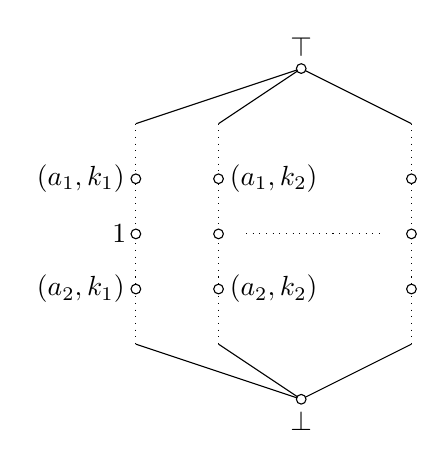
\begin{tikzpicture}[scale=0.70]
        \draw (3, 3) -- (0, 2);
        \draw[dotted] (0, 2) -- (0, -2);
        \draw (0, -2) -- (3, -3);
        \draw (3, 3) -- (1.5, 2);
        \draw[dotted] (1.5, 2) -- (1.5, -2);
        \draw (1.5, -2) -- (3, -3);
        \draw (3, 3) -- (5, 2);
        \draw[dotted] (5, 2) -- (5, -2);
        \draw (5, -2) -- (3, -3);
        \draw[dotted] (2, 0) -- (4.5, 0);

        \filldraw [color = black, fill = white] (3, 3) circle(2.5pt)
            (3, 3.4) node {$\top$};
        \filldraw [color = black, fill = white] (3, -3) circle(2.5pt)
            (3, -3.4) node {$\bot$};
        \filldraw [color = black, fill = white] (0, 1) circle(2.5pt)
            (-1, 1) node {$(a_1, k_1)$};
        \filldraw [color = black, fill = white] (0, 0) circle(2.5pt)
            (-0.3, 0) node {$1$};
        \filldraw [color = black, fill = white] (0, -1) circle(2.5pt)
            (-1, -1) node {$(a_2, k_1)$};

        \filldraw [color = black, fill = white] (1.5, 1) circle(2.5pt)
            (2.5, 1) node {$(a_1, k_2)$};
        \filldraw [color = black, fill = white] (1.5, 0) circle(2.5pt);
        \filldraw [color = black, fill = white] (1.5, -1) circle(2.5pt)
            (2.5, -1) node {$(a_2, k_2)$};

        \filldraw [color = black, fill = white] (5, 1) circle(2.5pt);
        \filldraw [color = black, fill = white] (5, 0) circle(2.5pt);
        \filldraw [color = black, fill = white] (5, -1) circle(2.5pt);
    \end{tikzpicture}
    \end{center}
    \caption{$\mathbf{R}_{\varphi, f}$}
    \label{f: semidirect}
    \end{figure}
\end{frame}

\begin{frame}
    \begin{block}{Theorem}
        If $\mathbf{K}$ is a cancellative monoid, $\mathbf{A}$ is a residuated chain, $\varphi: \mathbf{K} \rightarrow \m {ResEnd}(\mathbf{A})$ is a map, and $f: K \times K \rightarrow A$ is a $2$-cocycle with respect to $\m K$, $\m A$ and $\varphi$, then $\mathbf{R}_{\varphi, f}$ is the reduct of a residuated lattice.
    \end{block}
    \pause

    \begin{block}{Corollary}
        If the $2$-cocycle $f$ is trivial, then $\varphi$ is a monoid homomorphism and $(A \times K, \cdot, (1, 1))$ is a semidirect product of $\m A$ and $\m K$.
        In this case, we denote $\m R_{\varphi, f} = \m A \rtimes^b_{\varphi} \m K$.
    \end{block}
    \pause
    \medskip

    \begin{center}
        {\Large Thank you!}
    \end{center}
    
    
\end{frame}

\end{document} 
